%!TEX TS-program = xelatex
%!TEX encoding = UTF-8 Unicode
% !TEX root = ../../metm.tex

\begin{refsection}

\section{Riverberi Digitali}
\thispagestyle{empty}

Nonostante l'acustica architettonica sia stata parte integrante della
progettazione di strutture per millenni, la materia ha ottenuto una base
scientifica solida solo ai primi del novecento per opera di Wallace Sabine.
La definizione del tempo di riverbero da parte di Sabine è il punto di partenza
anche nella letteratura sulla modellazione digitale dell'effetto ad opera di
Manfred Schroeder. Con Sabine il tempo di riverbero può essere descritto,
misurato, previsto. Tutto quello che sappiamo fare oggi continua ad attingere
alle sue ricerce.

\subsection{Sabine}

\subsection{Natural Sounding Artificial Reverberation}

% STAMPA DEI BARPLOT
% bar(faustout);
% xlim ([0 10]);
% set(gca,'fontname','fira', "fontsize", 12);
% grid on;
% xlabel('Time (samples)');
% ylabel('Amplitude');
% set(gca,'XTick',0:1:10);
% print -dpng dfl.png

Il primo oggetto che Schroeder descrive è una linea di ritardo retro-alimentata
da una linea di \emph{feedback} controllato dal coefficiente $g < 1$.

\begin{figure}[ht]
  \centering
  \includegraphics[width=\textwidth]{CAPITOLI/0500/IMG/dfl.png}
  \caption[]{Delay in Feedback Loop. Schroeder, 1962.}
  \label{schroeder:dfl}
\end{figure}

Il blocco prevede un valore di ritardo $t$ che può avere diversi significati,
come cercherò di spiegare più avanti.

Il codice Faust per la realizzazione di tale oggetto è il seguente.

\lstinputlisting{CAPITOLI/0500/CODES/REV/dfl.dsp}

Il codice di descrizione della funzione è presente tutto in riga tre, la quale
può essere smontata in diversi blocchi per comprenderne la sintassi. Il blocco di
ritardo \texttt{delay} deve essere inizializzato con il valore massimo utilizzabile in
campioni. L'impostazione \texttt{SR/2} permette di avere almeno mezzo secondo
a qualsiasi requenza di campionamento. Il tempo $t$ di ritardo effettivo, in
quanto unità al campione, deve essere necessariamente un intero, motivo per cui
la variabile in entrata $t$ viene passata per una funzione \texttt{int}.

L'uscita del blocco di ritardo viene prelevata prima dell'uscita dal filtro e
reindirizzata all'entrata, in somma con l'entrata del filtro, adeguatamente
controlla dal coeffficiente $g < 1$.

\begin{figure}[t!]
  \centering
  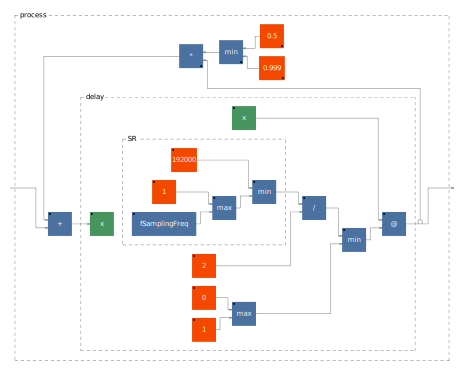
\includegraphics[width=\textwidth]{CAPITOLI/0500/CODES/REV/dfl-svg/process.pdf}
  \caption[]{Delay in Feedback Loop. Implementazione Faust.}
  \label{faust:dfl}
\end{figure}

\begin{figure}[ht]
  \centering
  \includegraphics[width=\textwidth]{CAPITOLI/0500/IMG/dfl-ir.png}
  \caption[]{Schroeder dfl impulse response.}
  \label{schroeder:dflir}
\end{figure}

\begin{figure}[ht]
  \centering
  \includegraphics[width=\textwidth]{CAPITOLI/0500/CODES/REV/dfl.png}
  \caption[]{Faust dfl impulse response.}
  \label{faust:dflir}
\end{figure}

Schoreder fornisce una chiara descrizione del funzionamento temporale del filtro
ed attraverso un diagramma ne mostra la risposta all'impulso. La figura
\ref{schroeder:dflir} mostra il comportamento del filtro ad un tempo $t$
consistente in ripetizioni successive per multipli interi $2t$, $3t$ \ldots fino
al completo esaurimento dell'ampiezza per opera del coefficiente scalare $g$.



Lo stesso si può dire del nostro modello: il tempo di ritardo $t$ regola le
nuove occorrenze dell'impulso generate dal
circuito di retroazione scalate dal coefficiente $g$. Pur avendo creato un
diagramma a blocchi \ref{faust:dfl} piuttosto fedele al modello di Schroeder di
figura \ref{schroeder:dfl}, la risposta all'impulso del nostro filtro merita
uno sguardo di analisi e un'attenta riflessione.



La risposta all'impulso di figura \ref{faust:dflir} è stata generata impostando
le variabili $t=1$ (un campione di ritardo) e $g=0.5$ (ampiezza dimezzata ad
ogni giro di feedback). Ci si aspetta quindi un comportamento molto simile a
quello descritto da Schroeder, per una successione di multipli di $1$ dovremmo
avere il primo impulso nella posizione $n[1]$ con ampiezza $a=1$ (non scalata,
non l'impulso non è ancor transitato nel ciclo di ffeedback). Il secondo impulso
dovrebbe essere posizionato subito dopo il primo, nella posizione $n[2]$ con
ampiezza $a=0.5$, e cosi proseguendo. Tuttavia, osservando l'indicizzazione dei
campioni sull'asse delle ascisse della figura \ref{faust:dflir} si può constatare
che in realtà il nostro filtro sta impiegando due campioni per ogni ciclo
impulsivo in luogo di uno, posizionando gli impulsi per $2t$.

La motivazione di questa differenza è nascosta dietro al significato del diagramma
a blocchi di entrambe le rappresentazioni. Nella prima, quella originaria di Schroeder,
il punto di prelievo del segnale per il ciclo di feedback è a tempo zero, ovvero
linea che porta il segnale dall'uscita del blocco di ritardo all'entrata della
somma è istantanea. Nella descrizione algoritmica di faust mediante diagramma
a blocchi invece l'operatore $~$ produce contestualmente al prelievo del segnale,
un inevitabile campione di ritardo. La linea di ricircolo quindi, nel momento
in cui alimenta il blocco di ritardo, porta già un campione di ritardo su quello
corrente.

La correzione di questo filtro per ottenere il comportamento prospettato da Schroeder
consiste nel sottrarre il campione di ritardo, prodotto dalla ricorsione, alla
variabile $t$ con $t-1$. Questo tipo di intervento per $t=$ produrrà $t=1-1=0$
ovvero zero campioni di ritardo all'uscita, un campione, come richiesto,
scalato in $g$ all'entrata della somma di ricircolo. Questo tipo di operazione
crea però un offset temporale in quanto la sequenza di campioni ritardati, ora
corretta, si trova in uscita un campione prima (ritardo zero) di quello richiesto.
Anche questa problematica è risolvibile inserendo un ulteriore campione di ritardo
\texttt{mem} all'uscita dell'algoritmo, in modo da bilanciare l'intera sequenza
temporale.

\lstinputlisting{CAPITOLI/0500/CODES/REV/dflc.dsp}

La risposta all'impulso del filto corretto è ora coerente con le aspettative.

\begin{figure}[ht]
  \centering
  \includegraphics[width=\textwidth]{CAPITOLI/0500/CODES/REV/dflc.png}
  \caption[]{Faust dfl impulse response.}
  \label{faust:dflir}
\end{figure}

Il filtro appena costruito può operare tempi di ritardo tra $1$ e \emph{Nyquist}.
Questo comportamento può portare a diversi risultati sonori, dal più diretto
ritardo di una quantità di campioni indicata con $g=0$, oppure ad un filtraggio di componenti
spettrali in funzione di $t$ e $g$.

\begin{figure}[h]
  \centering
  \includegraphics[width=\textwidth]{CAPITOLI/0500/IMG/dfl-fr.png}
  \caption[]{Schroeder dfl risposta in requenza, \emph{”somigliante ad un pettine”}.}
  \label{schroeder:dflffr}
\end{figure}

\begin{quote}
  The amplitude-frequency responce has the appearance of a comb with periodic
  maxima and minima\ldots It is these peaks and valleyys which impart the undesidered
  “colored” qualityy to sound reverberated by devices like that.
\end{quote}



\printbibliography
\end{refsection}
